 \part{Experiments}

\chapter{Benchmark POMDPs}

UVOD DO PROBLEMU< PROC JSME JE VYRALI< KDE JSOU ULOZENE ATD

\section{Domains}

In this chapter, we introduce benchmark problems for both MDP and POMDP solvers. We have come up with custom, straightforward, dynamically sized problems sufficient for our validations of MDP solvers. On the other hand, the POMDPs are still actively researched. Examples of POMDP benchmark problems are at \cite{cassandra_1999}. Problems that we use were introduced in \cite{Littman}. The selected POMDP benchmark problems are implemented using the \textit{POMDPs.jl} interface in the \textit{POMDPPolicies.jl} package. In these benchmark problems, we have changed the definition of transitions from terminal states. In \cite{Littman} the author restarts the problem with the uniform transition to non-terminal states. In our implementation, we define the transitions from terminal states as deterministic transitions to themselves. 


\subsection{1D Grid}
Custom MDP 1D grid problem with custom number of states with terminal states on both ends. The agent can execute two actions (left and right) with a 30\% chance of executing the wrong one. For each action, the agent pays one point, and for reaching the terminal state, the agent receives ten points. 

\begin{figure}[ht]
\caption{1D Grid environment}
\centering
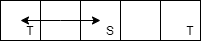
\includegraphics[scale=0.5]{pictures/1D_grid.png}
\end{figure}

\subsection{Pyramid}
Custom pyramid-like problem designed specifically for Finite Horizon MDP solvers. Starting in the first stage with 1 state, the pyramid problem grows "downward", growing an additional state in each stage (the first stage has \textit{1} state, ..., n$^{th}$ stage has \textit{n} states). The Pyramid MDP has two possible actions, moving down-left or down-right. Optionally, the user can define additional terminal states. By default the terminal states are contained in the last (\textit{horizon + 1}) stage. The rewards and costs are the same as in the 1D Grid problem.

\begin{figure}[ht]
\caption{Pyramid environment}
\centering
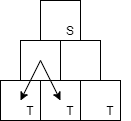
\includegraphics[scale=0.5]{pictures/Pyramid.png}
\end{figure}

\subsection{Mini Hallway}

Small navigation problem called Mini Hallway \cite{Littman} consisting of 13 states. The environment consists of 3 rooms with four orientations and a 4$^{th}$ terminal room denoted by a star. The agent can receive nine observations (relative locations of surrounding walls) and execute three actions (forward, rotate left, rotate right.
The problem models a hallway with a robot whose task is to enter the room marked with the star for which the agent gets one point. The actions are costless. The transitions and observations are deterministic. The initial state belief is uniformly distributed over all twelve non-terminal states.
\begin{figure}[ht]
\caption{Mini Hallway environment}
\centering
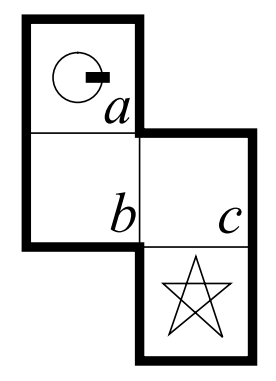
\includegraphics[scale=0.5]{pictures/MiniHallway.png}
\end{figure}

\subsection{Hallway}

Middle-sized navigation problem Hallway \cite{Littman} consisting of 60 states. The environment consists of 14 rooms with four orientations each and one room with 4 terminal states. Other than that, the model contains 21 observations (possible combinations of wall presence, a star denoting the terminal states, and three numbered landmarks) and five actions (stay in place, move forward, turn right, turn left, turn around). Both transitions and observations are extremely noisy. For reaching the terminal state, the agent receives one point. The agent does not pay for his actions. The initial state belief is uniformly distributed over all 56 non-terminal states.

\begin{figure}[ht]
\caption{A Hallway environment}
\centering
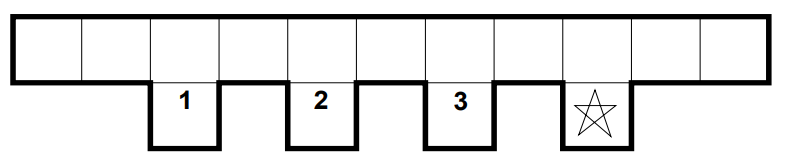
\includegraphics[scale=0.5]{pictures/hallway.png}
\end{figure}








\begin{table}[ht]
\centering
\begin{tabular}{||c c c c c c c||} 
 \hline
 Domain & $|S|$ & $|A|$ & $|\Omega|$ & Observability & Transitions & Observations \\
 \hline\hline
 1D Grid & custom & 2 & 0 & Fully Observable & Stochastic & Null \\
 Pyramid & custom & 2 & 0 & Fully Observable & Stochastic & Null \\
 MiniHallway & 13 & 3 & 9 & Partially Observable & Deterministic & Deterministic \\
 Hallway & 60 & 5 & 21 & Partially Observable & Stochastic & Stochastic \\
 \hline
\end{tabular}
\caption{Table to test captions and labels}
\label{TODO1}
\end{table}


% Tag????

\section{Validations and Benchmarks}

In the following validations and benchmarks, we are using algorithms implemented in the POMDPs.jl framework. All experiments were executed on a 2.6Ghz i7 CPU with four cores and 16GB RAM. The algorithms were not run in parallel, nor were they multi-threaded. Results for MDP solvers were evaluated using \textit{BenchmarkTools.jl} package. The algorithm stopped either after evaluating 10 000 algorithm executions or after 100 seconds. The POMDP solvers' policies were evaluated for each iteration separately, and for each of them, we simulated its behavior using \textit{POMDPSimulators.jl} package 10 000 times.

\subsection{Finite Horizon Value Iteration}
The Finite Horizon Value Iteration was evaluated against the Infinite Horizon Value Iteration with staged 1D Grid (transformed to Finite Horizon) problem and staged Pyramid Problem consecutively. Both solvers have guaranteed convergence. That is, the Finite Horizon Value Iteration offers a one-pass solution, and the Infinite Horizon Value Iteration converges after an unknown number of iterations. Furthermore, the Infinite Horizon Value Iteration updates the value function of all states in each stage in each iteration. On the other hand, the Finite Horizon Value Iteration only iterates over the states in the given stage and ends after \textit{horizon} iterations.

In the 1D Grid problem, we used problems with 5, 11, 25, 51, and 101 states in each stage. The terminal states were at the edges and the starting point in the middle. In this problem, it takes the agent \textit{(n - 1) / 2} actions to get to one of the terminal states. It takes the same amount of iterations to update the value functions of all states correctly. Thus, for solving staged 1D Grid problem, the Finite Horizon Value Iteration algorithm requires ((n - 1) / 2) $\times$ ((n - 1) / 2) \textit{(for number of iterations times less states in each iteration)} / 2 \textit{(for each iteration, the Finite Horizon Value Iteration needs both old and a new stage, thus doubling its memory requirements)} less memory. 

The benchmarking results are validating our results. For example, for 51 states, it would take 25 iterations with 25 times more states in each of them divided by two. Thus, the memory requirement of Finite Horizon Value Iteration is 312.5 times slower than the memory required for the Infinite Horizon Value Iteration used on the staged 1D Grid problem. 312.5 times reduction equals to reduction to 0.32 \%. The experiment in Table \ref{table:memory_1D_MDP_VI} validates our prediction. Similar trends can be seen in Table \ref{table:time_1D_MDP_VI}. The dependence between the number of states of one stage in Finite Horizon 1D Grid Problem and the time needed to solve the problem is in Figure \ref{graph1}.



\begin{figure}[ht]
\centering
\incfig{MDP_1D_VI}
\caption{Comparison of Finite and Infinite Horizon \\ Value Iteration solvers on various sized staged 1D Grid problem}
\label{graph1}
\end{figure}


\begin{table}[ht]
\centering
\begin{tabular}{l *{3}{S[table-format=1.3]} *{2}{S[table-format=3.3]}}
\toprule
 Number of states & \multicolumn{1}{c}{5} & \multicolumn{1}{c}{11} & \multicolumn{1}{c}{25} & \multicolumn{1}{c}{51} & \multicolumn{1}{c}{101}  \\
 \midrule
 IH VI [ms] & 0.165 & 0.933 & 10.850 & 218.452 & 2115.453 \\
 FH VI [ms] & 0.014 & 0.089 & 0.289 & 1.045 & 3.466 \\
 \midrule
 Improvement [$\times$]& 11.8 & 10.5 & 37.6 & 209.0 & 610.3 \\
  \bottomrule
\end{tabular}
\centering
\caption{Mean solving time comparison of Finite Horizon \\ and Infinite Horizon Value iteration of various sized staged 1D Grid problem}
\label{table:time_1D_MDP_VI}
\end{table}


\begin{table}[ht]
\centering
\begin{tabular}{l *{3}{S[table-format=1.3]} *{2}{S[table-format=3.3]}}
 \toprule
   Number of states & \multicolumn{1}{c}{5} & \multicolumn{1}{c}{11} & \multicolumn{1}{c}{25} & \multicolumn{1}{c}{51} & \multicolumn{1}{c}{101}  \\
  \midrule
 IH VI [MB] & 0.044 & 1.118 & 17.904 & 313.767 & 4336.078 \\
 FH VI [MB] & 0.009 & 0.051 & 0.225 & 0.987 & 3.768 \\
  \midrule
 Reduced to [\%]& 20.34 & 4.54 & 1.25 & 0.31 & 0.08 \\
  \bottomrule
\end{tabular}
\caption{Memory consumption comparison of Finite Horizon \\ and Infinite Horizon Value iteration of various sized staged 1D Grid problem}
\label{table:memory_1D_MDP_VI}
\end{table}


In the Pyramid problem, instead of the number of states, we used the number of horizons, as those numbers are equal in this problem. The Pyramid MDP problem requires less memory than the 1D Grid problem, and thus we extended our validations to 5, 11, 25, 51, 101, 251, 501 horizons. Unlike the 1D Grid MDP, the agent in Pyramid MDP needs to execute \textit{number of horizons} actions to get into the terminal state. The memory requirements in Table \ref{table:memory_Pyramid_MDP_VI} show less memory reduction. The problem's pyramid-like state-space causes less memory reduction as the problem consists only of the states to which the agent can get. As expected, the specialized Finite Horizon Value Iteration outperforms the general Infinite Horizon Value Iteration in terms of performance as well. The time-wise performances are shown in Table \ref{table:time_Pyramid_MDP_VI}. The distribution of time-wise performances for each size of the problem is in Figure \ref{graph2}.

\begin{figure}[ht]
    \centering
    \incfig{MDP_Pyramid_VI}
    \caption{Comparison of Finite and Infinite Horizon \\ Value Iteration solvers on staged Pyramid problem with different horizons}
    \label{graph2}
\end{figure}

\begin{table}[ht]
\centering
\begin{tabular}{l *{5}{S[table-format=1.3]} *{2}{S[table-format=3.3]}}
 \toprule
   Horizon & \multicolumn{1}{c}{5} & \multicolumn{1}{c}{11} & \multicolumn{1}{c}{25} & \multicolumn{1}{c}{51} & \multicolumn{1}{c}{101} & \multicolumn{1}{c}{251} & \multicolumn{1}{c}{501}  \\
  \midrule
 IH VI [ms] & 0.058 & 0.119 & 0.518 & 3.651 & 27.456 & 401.497 & 3289.083\\
 FH VI [ms] & 0.021 & 0.031 & 0.099 & 0.236 & 0.668 & 2.605 & 9.605 \\
  \midrule
 Improvement [$\times$]& 2.8 & 3.8 & 5.2 & 15.5 & 41.0 & 154.1 & 342.4 \\
 \bottomrule
\end{tabular}
\caption{Mean solving time comparison of Finite Horizon \\ and Infinite Horizon Value iteration of various sized staged Pyramid problem}
\label{table:time_Pyramid_MDP_VI}
\end{table}


% \backslashbox{solver}{no states}



% \backslashbox{solver}{no horizons}
\begin{table}[h]
\centering
\begin{tabular}{l *{7}{S[table-format=1.3]}}
 \toprule
   Horizon & \multicolumn{1}{c}{5} & \multicolumn{1}{c}{11} & \multicolumn{1}{c}{25} & \multicolumn{1}{c}{51} & \multicolumn{1}{c}{101} & \multicolumn{1}{c}{251} & \multicolumn{1}{c}{501}  \\
  \midrule
 IH VI [MB] & 0.011 & 0.028 & 0.096 & 0.376 & 1.481 & 6.923 & 23.574\\
 FH VI [MB] & 0.007 & 0.015 & 0.041 & 0.119 & 0.376 & 1.970 & 7.304 \\
  \midrule
 Reduced to [\%]& 59.0 & 52.6 & 42.7 & 31.8 & 25.4 & 28.5 & 31.0\\
 \bottomrule
\end{tabular}
\caption{Memory consumption comparison of Finite Horizon \\ and Infinite Horizon Value iteration of various sized staged Pyramid problem}
\label{table:memory_Pyramid_MDP_VI}
\end{table}




\subsection{Point-Based Value Iteration}
We formerly wanted to benchmark the FiVI against the PBVI. However, the PointBasedValueIteration.jl package did not contain a correctly implemented algorithm. This chapter serves as the validation of the correct algorithm implementation. We evaluated the PBVI against the SARSOP algorithm [TODO: reference]. The SARSOP is based on the PBVI, and as such, the PBVI can not outperform the SARSOP but can obtain a similar reward after longer solving.


In Figure \ref{graph3}, we can see that the PBVI starts with a decent 0.3 mean reward, then dips, and in the end reaches a similar reward as the SARSOP. In the beginning, the PBVI's explored space contains only a tiny part of the belief space. The starting reward can be awarded to $\alpha$-vector correctly executing an action corresponding to maximizing the value function of the belief unknown to the solver. The value function of those specific beliefs is not yet calculated, thus inaccurate. In the middle dip, the algorithm starts to explore the first most promising beliefs. The solver knows that the beliefs are promising but yet does not know which way to go. The solver finally explores the optimal path in the last iteration and gradually updates all other beliefs with new actions, obtaining the same reward as SARSOP.

The SARSOP leverages heuristics to explore the optimal state-space efficiently. The PBVI only does not. The use of heuristics results in PBVI being significantly slower than SARSOP. The advantage of heuristics highlights more than hundreds of times more efficient memory consumption of SARSOP.


\begin{figure}[ht]
    \centering
    \incfig{POMDP_Hallway_PBVI}
    \caption{Comparison of the expected reward depending on the length of problem solving between Point Based Value Iteration and SARSOP on the Hallway problem.}
    \label{graph3}
\end{figure}


\subsection{Finite Horizon Point-Based Value Iteration}
The FiVI algorithm is a great starting point for Finite Horizon POMDP solvers for POMDPs.jl. This section shows that the solver is correctly implemented and benchmarked against the previous section's PBVI algorithm. In the benchmark scenario, the FIVI easily dominates PBVI, the base solver for Infinite Horizon POMDPs. The other algorithms, such as SARSOP, can not be used, as they do not support the Finite Horizon POMDPs interface. 

We have benchmarked the FiVI and PBVI on the staged MiniHallway problem. MiniHallway offers a moderate problem for FiVI but is a significant problem in terms of size for PBVI. The choice of lesser staged problems as TigerPOMDP or BabyPOMDP from $POMDPPolicies.jl$ does not represent a suitable sized benchmark. On the other hand, the staged Hallway problem would take the PBVI hundreds or thousands of seconds to solve. 

We benchmark the MiniHallway problem with multiple choices for the horizon value. With multiple stages, we simulate multiple various-sized problems. The horizon values are 3, 6, 9. With the uniformly distributed initial belief, horizon 3 offers only a slight possibility for reaching terminal states. Horizon 6 is a middle-sized problem in which the agent has more steps to execute and improves its expected reward. Horizon 9 simulates a long-range problem, challenging for the PBVI solver.

In the first two benchmarks, we can see that the PBVI almost reaches a similar expected reward as the FiVI. However, the time needed to obtain such a policy is far greater. In the last benchmark, the PBVI does not solve the problem in the time limit and stops with the expected reward of 0.31. The FiVI, on the other hand, converges and obtains an expected reward of 0.58.

The most significant problem for leveraging the PBVI in Finite Horizons is that it starts with only an initial belief, and it has to expand its belief space iteratively. FiVI, on the other hand, starts with the initial belief and another \textit{|S|} beliefs in each stage. This way, the FiVI algorithm contains significantly more beliefs in its first stage, allowing it to solve problems significantly faster.

% \begin{table}[ht]
% \centering
% \begin{tabular}{||c c c c ||} 
%  \hline
%  {} & {} & PBVI & FiVI \\
%  \hline
%  MiniHallway & Expected Reward & 0.23 & 0.24 \\
%  h = 3 & Time (s) & 18.59 & 2.36 \\
%  \hline
%  MiniHallway & Expected Reward & 0.31 & 0.33\\
%  h = 6 & Time (s) & 90.45 & 30.52\\
%  \hline
%  MiniHallway & Expected Reward & 0.31 & 0.58\\
%  h = 9 & Time (s) & 279.69 & 37.59\\
%   \hline
% \end{tabular}
% \caption{Mean solving time comparison [ms]}
% \label{TODO8}
% \end{table}



\begin{table}[ht]
\centering
\begin{tabular}{l *{3}{S[table-format=3.3]} | *{3}{S[table-format=3.3]}}
 \hline
 {} & \multicolumn{3}{c|}{Expected reward} & \multicolumn{3}{c}{Time[s]} \\
 horizon  & \multicolumn{1}{c}{3} & \multicolumn{1}{c}{6} & \multicolumn{1}{c|}{9} & \multicolumn{1}{c}{3} & \multicolumn{1}{c}{6} & \multicolumn{1}{c}{9}\\
 \hline
 PBVI & 0.23 & 0.31 & 0.31 & 18.59 & 90.45 & 279.69 \\
 FiVI & 0.24 & 0.33 & 0.58 & 2.36 & 30.52 & 37.59 \\
 \bottomrule
\end{tabular}
\caption{Comparison of expected rewards and time needed to solve the problem with Finite Horizon or Infinite Horizon Value Iteration on MiniHallway Problem}
\label{TODO8}
\end{table}



% Finite Horizon - LB, GAP, Time TABLE -- ZATIM NEMAM VUCI CEMU POROVNAVAT
%                 - GAP vs Time Graf
                
% INFINITE horizon - reward vs time graf
%                 - Reward, \% Goal, |B|, Time Table
                
                

% kolikrat rzchlejsi  
% kolik iteraci
% kolik pameti
% kolik to trva


% aszmptoticka slozitost